% Options for packages loaded elsewhere
\PassOptionsToPackage{unicode}{hyperref}
\PassOptionsToPackage{hyphens}{url}
\documentclass[
]{article}
\usepackage{xcolor}
\usepackage{amsmath,amssymb}
\setcounter{secnumdepth}{-\maxdimen} % remove section numbering
\usepackage{iftex}
\ifPDFTeX
  \usepackage[T1]{fontenc}
  \usepackage[utf8]{inputenc}
  \usepackage{textcomp} % provide euro and other symbols
\else % if luatex or xetex
  \usepackage{unicode-math} % this also loads fontspec
  \defaultfontfeatures{Scale=MatchLowercase}
  \defaultfontfeatures[\rmfamily]{Ligatures=TeX,Scale=1}
\fi
\usepackage{lmodern}
\ifPDFTeX\else
  % xetex/luatex font selection
\fi
% Use upquote if available, for straight quotes in verbatim environments
\IfFileExists{upquote.sty}{\usepackage{upquote}}{}
\IfFileExists{microtype.sty}{% use microtype if available
  \usepackage[]{microtype}
  \UseMicrotypeSet[protrusion]{basicmath} % disable protrusion for tt fonts
}{}
\makeatletter
\@ifundefined{KOMAClassName}{% if non-KOMA class
  \IfFileExists{parskip.sty}{%
    \usepackage{parskip}
  }{% else
    \setlength{\parindent}{0pt}
    \setlength{\parskip}{6pt plus 2pt minus 1pt}}
}{% if KOMA class
  \KOMAoptions{parskip=half}}
\makeatother
\usepackage{graphicx}
\makeatletter
\newsavebox\pandoc@box
\newcommand*\pandocbounded[1]{% scales image to fit in text height/width
  \sbox\pandoc@box{#1}%
  \Gscale@div\@tempa{\textheight}{\dimexpr\ht\pandoc@box+\dp\pandoc@box\relax}%
  \Gscale@div\@tempb{\linewidth}{\wd\pandoc@box}%
  \ifdim\@tempb\p@<\@tempa\p@\let\@tempa\@tempb\fi% select the smaller of both
  \ifdim\@tempa\p@<\p@\scalebox{\@tempa}{\usebox\pandoc@box}%
  \else\usebox{\pandoc@box}%
  \fi%
}
% Set default figure placement to htbp
\def\fps@figure{htbp}
\makeatother
% definitions for citeproc citations
\NewDocumentCommand\citeproctext{}{}
\NewDocumentCommand\citeproc{mm}{%
  \begingroup\def\citeproctext{#2}\cite{#1}\endgroup}
\makeatletter
 % allow citations to break across lines
 \let\@cite@ofmt\@firstofone
 % avoid brackets around text for \cite:
 \def\@biblabel#1{}
 \def\@cite#1#2{{#1\if@tempswa , #2\fi}}
\makeatother
\newlength{\cslhangindent}
\setlength{\cslhangindent}{1.5em}
\newlength{\csllabelwidth}
\setlength{\csllabelwidth}{3em}
\newenvironment{CSLReferences}[2] % #1 hanging-indent, #2 entry-spacing
 {\begin{list}{}{%
  \setlength{\itemindent}{0pt}
  \setlength{\leftmargin}{0pt}
  \setlength{\parsep}{0pt}
  % turn on hanging indent if param 1 is 1
  \ifodd #1
   \setlength{\leftmargin}{\cslhangindent}
   \setlength{\itemindent}{-1\cslhangindent}
  \fi
  % set entry spacing
  \setlength{\itemsep}{#2\baselineskip}}}
 {\end{list}}
\usepackage{calc}
\newcommand{\CSLBlock}[1]{\hfill\break\parbox[t]{\linewidth}{\strut\ignorespaces#1\strut}}
\newcommand{\CSLLeftMargin}[1]{\parbox[t]{\csllabelwidth}{\strut#1\strut}}
\newcommand{\CSLRightInline}[1]{\parbox[t]{\linewidth - \csllabelwidth}{\strut#1\strut}}
\newcommand{\CSLIndent}[1]{\hspace{\cslhangindent}#1}
\setlength{\emergencystretch}{3em} % prevent overfull lines
\providecommand{\tightlist}{%
  \setlength{\itemsep}{0pt}\setlength{\parskip}{0pt}}
\usepackage{bookmark}
\IfFileExists{xurl.sty}{\usepackage{xurl}}{} % add URL line breaks if available
\urlstyle{same}
\hypersetup{
  pdftitle={AGENTE CONVERSACIONAL PARA INTERAÇÃO APRIMORADA EM SISTEMAS},
  hidelinks,
  pdfcreator={LaTeX via pandoc}}

\title{\textbf{AGENTE CONVERSACIONAL PARA INTERAÇÃO APRIMORADA EM
SISTEMAS}}
\author{}
\date{}

\begin{document}
\maketitle

\subsubsection{Artigo em produção - Checklist de
produção}\label{artigo-em-produuxe7uxe3o---checklist-de-produuxe7uxe3o}

\begin{itemize}
\tightlist
\item[$\square$]
  Edição do artigo

  \begin{itemize}
  \tightlist
  \item[$\boxtimes$]
    Aplicar ABNT
  \item[$\square$]
    Aplicar formatação da SATC
  \end{itemize}
\item[$\square$]
  Escrita

  \begin{itemize}
  \tightlist
  \item[$\square$]
    Resumo

    \begin{itemize}
    \tightlist
    \item[$\boxtimes$]
      Esqueleto
    \item[$\square$]
      Revisão após finalizar o artigo
    \end{itemize}
  \item[$\boxtimes$]
    Introdução (preciso de umas referências)
  \item[$\square$]
    Material e métodos

    \begin{itemize}
    \tightlist
    \item[$\boxtimes$]
      Abordagem geral
    \item[$\boxtimes$]
      Materiais
    \item[$\square$]
      Métodos

      \begin{itemize}
      \tightlist
      \item[$\square$]
        Procedimento experimental de cada alternativa
      \end{itemize}
    \end{itemize}
  \item[$\square$]
    Resultados e discussão
  \item[$\square$]
    Considerações finais
  \item[$\square$]
    Referências

    \begin{itemize}
    \tightlist
    \item[$\boxtimes$]
      Formatar ABNT
    \end{itemize}
  \end{itemize}
\end{itemize}

\textbf{Lucas de Castro Zanoni}\footnote{Graduando em Engenharia de
  software no semestre letivo de 2024-2. E-mail:
  castro.lucas290@gmail.com}

\textbf{Thyerri Fernandes Mezzari}\footnote{Professor do Centro
  Universitário UniSATC E-mail: thyerri.mezzari@satc.edu.br}

Resumo: Este trabalho apresenta o desenvolvimento de um agente
conversacional baseado em inteligência artificial para aprimorar a
interação entre usuários e sistemas. Utilizando técnicas avançadas de
processamento de linguagem natural, o agente proposto visa simplificar a
comunicação em interfaces complexas, proporcionando uma experiência
digital unificada e adaptável às necessidades dos usuários. A
metodologia inclui o desenvolvimento, implementação e avaliação do
agente em ambientes reais de uso. Os resultados demonstram que a solução
proposta contribui significativamente para a melhoria da acessibilidade
e usabilidade dos sistemas, reduzindo barreiras de interação e
promovendo uma comunicação mais fluida e intuitiva.

\textbf{Palavras-chaves:} agente conversacional, interação, sistema,
inteligência artificial.

\section{1 INTRODUÇÃO}\label{introduuxe7uxe3o}

A evolução das interfaces de usuário tem gerado uma diversidade de
padrões de design e usabilidade, resultando frequentemente em barreiras
para a plena acessibilidade e interação dos usuários com os sistemas
digitais. Com o aumento da complexidade do frontend e a multiplicidade
de paradigmas de interação, muitos usuários enfrentam dificuldades
significativas para utilizar efetivamente as funcionalidades oferecidas
pelos sistemas computacionais modernos (RAPP et al., 2018) (KOCABALLI et
al., 2019).

Nesse cenário, os agentes conversacionais baseados em inteligência
artificial emergem como uma alternativa promissora para simplificar a
comunicação entre humanos e máquinas, oferecendo uma camada
intermediária de interação que pode traduzir comandos em linguagem
natural para ações específicas no sistema.

Estudos recentes têm demonstrado que agentes conversacionais podem
aprimorar significativamente a experiência do usuário ao simplificar
interações com sistemas complexos (FAST et al., 2017). Além disso, a
implementação de interfaces baseadas em linguagem natural tem mostrado
potencial para melhorar a usabilidade em contextos domésticos e
inteligentes, reduzindo o tempo e o esforço necessários para completar
tarefas complexas (GUO et al., 2024). Ademais, tais interfaces oferecem
vantagens consideráveis em termos de acessibilidade, permitindo uma
comunicação mais inclusiva e adaptável a usuários com diferentes
necessidades especiais (LISTER et al., 2020) (DENG, 2023).

A problemática central desta pesquisa reside na questão: de que forma um
agente conversacional baseado em IA pode potencializar a interação entre
usuários e sistemas, promovendo uma comunicação fluida mesmo em
ambientes com interfaces complexas? Essa pergunta reflete a necessidade
crescente de soluções que democratizem o acesso à tecnologia, reduzindo
a curva de aprendizado necessária para a utilização de sistemas
especializados e tornando-os mais acessíveis para diferentes perfis de
usuários.

Adicionalmente, trabalhos recentes indicam que avanços na arquitetura de
modelos de IA, como o uso de transformers sem camadas de normalização,
podem influenciar positivamente o desempenho e a eficiência desses
agentes (ZHU et al., 2025).

A relevância deste estudo evidencia-se pelo potencial transformador que
os agentes conversacionais representam para a área de interação
humano-computador. Ao implementar um sistema intermediário capaz de
interpretar linguagem natural e traduzi-la em ações específicas dentro
de um sistema, cria-se uma ponte que permite aos usuários interagir de
forma mais intuitiva e natural com as tecnologias digitais. Esta
abordagem tem o potencial de mitigar as barreiras impostas por
interfaces complexas, contribuindo para uma maior inclusão digital e
para a melhoria da experiência do usuário em diversos contextos de
aplicação.

\section{2 PROCEDIMENTO EXPERIMENTAL}\label{procedimento-experimental}

Este trabalho adota uma abordagem metodológica estruturada em múltiplas
etapas para investigar e avaliar diferentes métodos de integração entre
agentes conversacionais baseados em LLMs (Large Language Models) e
sistemas computacionais. A pesquisa se desenvolve através de uma análise
comparativa de quatro abordagens distintas de integração, cada uma com
suas características, vantagens e limitações específicas.

O processo investigativo inicia-se com uma revisão sistemática da
literatura sobre integrações entre LLMs e sistemas, estabelecendo uma
base teórica sólida para a análise subsequente. Em seguida, são
exploradas quatro abordagens principais de integração: (1) conexão
direta com banco de dados, permitindo consultas e manipulações diretas;
(2) integração via plugins ORM, facilitando o acesso através de camadas
de abstração existentes; (3) integração via API/Swagger, utilizando
interfaces padronizadas de comunicação; e (4) integração via Model
Context Protocol (MCP), explorando um paradigma emergente de comunicação
entre LLMs e sistemas.

Para cada abordagem, será desenvolvida uma prova de conceito que
demonstre sua viabilidade técnica e permita uma avaliação objetiva de
seus aspectos funcionais e não-funcionais. A avaliação seguirá critérios
predefinidos, incluindo desempenho, segurança, facilidade de
implementação, manutenibilidade e experiência do usuário. Os resultados
serão documentados e analisados de forma sistemática, permitindo uma
comparação objetiva entre as diferentes abordagens.

\subsection{2.1 MATERIAIS}\label{materiais}

Para garantir a rigorosidade científica e a reprodutibilidade dos
experimentos conduzidos neste estudo, é essencial uma seleção criteriosa
dos materiais e ferramentas utilizados. Esta seção detalha os recursos
específicos empregados na condução desta pesquisa, justificando sua
escolha baseada na eficiência, popularidade, robustez e aplicabilidade
prática dentro do contexto dos agentes conversacionais e integração de
sistemas.

\subsubsection{2.1.1 NODE.JS PARA DESENVOLVIMENTO DAS PROVAS DE
CONCEITO}\label{node.js-para-desenvolvimento-das-provas-de-conceito}

Node.js foi escolhido como plataforma principal para o desenvolvimento
das provas de conceito devido à sua comprovada eficácia na integração de
sistemas baseados em inteligência artificial (IA), especialmente com
agentes conversacionais e Large Language Models (LLMs). A plataforma é
amplamente adotada devido à sua arquitetura orientada a eventos e
capacidade de gerenciar eficientemente múltiplas conexões simultâneas,
essencial para aplicações que exigem respostas rápidas em tempo real
(CHEREDNICHENKO et al., 2024).

O Hugging Face fornece bibliotecas JavaScript específicas compatíveis
com Node.js, como o \texttt{@huggingface/inference}, permitindo acesso
direto a mais de 100 mil modelos pré-treinados com suporte a TypeScript.
Isso simplifica significativamente a integração com IA, destacando a
robustez técnica e facilidade de adoção do Node.js em aplicações
modernas (FACE, 2024).

Grandes empresas também reforçam a relevância de Node.js ao
disponibilizarem SDKs específicos, como o da IBM para o Watsonx, lançado
em 2023. Este SDK facilita o uso direto de modelos generativos robustos
da IBM em aplicações Node.js, destacando sua relevância estratégica no
ambiente empresarial (IBM, 2023).

Adicionalmente, a documentação oficial do Node.js ressalta sua
capacidade superior de lidar com streaming de dados através de streams e
pipelines. Essa funcionalidade permite transmitir resultados
incrementais de IA aos clientes com baixa latência, tornando-o ideal
para chatbots e serviços em tempo real que dependem de respostas
imediatas (NODE.JS, 2024).

Por fim, relatórios da Red Hat destacam que o uso eficiente da
arquitetura assíncrona do Node.js possibilita a criação de agentes
baseados em LLMs com alta performance e escalabilidade. Isso garante um
gerenciamento eficiente de múltiplas operações paralelas, essencial para
aplicações intensivas em IA e integração com APIs externas (BLOG, 2024).

\subsubsection{2.1.2 TESTES END-TO-END
(E2E)}\label{testes-end-to-end-e2e}

O Framework de Gerenciamento de Riscos de IA do NIST (OPREA; VASSILEV,
2023) destaca a importância de avaliar o desempenho de sistemas de IA de
forma abrangente, defendendo que testes de integração devem avaliar os
sistemas de ponta a ponta para identificar erros de integração e
garantir a precisão das respostas em cenários realistas. Testes
rigorosos como esses não apenas identificam problemas de integração, mas
também asseguram às partes interessadas que o sistema se comporta
conforme o esperado em condições do mundo real.

A injeção de prompt representa um risco significativo em implantações de
LLMs em nosso cenário, no qual o modelo possui acesso a dados e sistemas
potencialmente críticos, incluindo, ocasionalmente, conexões diretas com
dados brutos de banco de dados. O guia de riscos da OWASP (JOHN et al.,
2025) classifica a injeção de prompt como uma ameaça crítica à
segurança, destacando a necessidade de procedimentos de teste rigorosos
para garantir que agentes conversacionais baseados em LLMs não revelem
inadvertidamente dados sensíveis ou contornem restrições do sistema
quando expostos a entradas maliciosas. Recentemente, Wu et al.~(2023)
(WU et al., 2023) demonstraram que ataques de jailbreak --- um tipo
avançado de injeção de prompt --- podem burlar as salvaguardas éticas de
modelos como o ChatGPT em até 67\% dos casos, gerando conteúdos
prejudiciais como extorsão e desinformação.

Com isso em mente, o uso de testes E2E pode ser utilizado para avaliar a
resiliência da implementação ao simular entradas adversárias, processo
conhecido como red teaming. Segundo Inie et al.~(2025) (INIE; STRAY;
DERCZYNSKI, 2025), o red teaming desafia sistematicamente sistemas de IA
com prompts adversários projetados para testar seus limites e mecanismos
de segurança. Ao encapsular consultas do usuário com lembretes de
responsabilidade ética (e.g., ``Você deve ser um ChatGPT responsável''),
o método reduziu a taxa de sucesso de jailbreaks para 19\%, mantendo a
funcionalidade padrão do modelo --- um resultado validado através de
testes E2E em 540 cenários adversarialmente projetados (WU et al.,
2023).

Testes de robustez, como os propostos pelo framework CheckList (RIBEIRO
et al., 2020), complementam ainda mais os testes E2E ao variar
sistematicamente as entradas --- como paráfrases, negações ou ruído ---
para avaliar a consistência e a precisão do modelo em diferentes
cenários. Esse método garante que sistemas baseados em LLM lidem de
forma confiável com interações diversas dos usuários, atributo essencial
para manter a confiança dos usuários e a estabilidade operacional,
especialmente em aplicações críticas de negócios ou voltadas à
segurança.

\subsubsection{2.1.3 MODELOS DE LINGUAGEM DE GRANDE ESCALA
(LLMs)}\label{modelos-de-linguagem-de-grande-escala-llms}

Os modelos de linguagem (LLMs), incluindo tecnologias como OpenAI GPT,
Anthropic e modelos disponibilizados pela Google, são essenciais neste
estudo devido à sua capacidade de interpretar e gerar linguagem natural
de forma avançada e eficaz. Estes modelos foram selecionados por sua
performance comprovada e ampla adoção em pesquisas acadêmicas e no
mercado corporativo, proporcionando um sólido embasamento para as
funcionalidades de interação do agente conversacional.

\paragraph{2.1.3.1 HISTÓRICO DO DESENVOLVIMENTO DE LLMS
(2018--2023)}\label{histuxf3rico-do-desenvolvimento-de-llms-20182023}

Nos últimos cinco anos, os Modelos de Linguagem de Grande Escala (LLMs)
evoluíram rapidamente, a partir da arquitetura Transformer. O lançamento
do BERT (2018) mostrou avanços em compreensão textual, enquanto a série
GPT demonstrou fortes capacidades generativas. O GPT-3 (2020), com 175
bilhões de parâmetros, evidenciou habilidades emergentes de aprendizado
com poucos exemplos (few-shot), ampliando o escopo de tarefas possíveis
por meio de simples instruções em linguagem natural (BROWN et al.,
2020).

A partir de 2022, o foco da pesquisa passou a ser o aprimoramento do
raciocínio e alinhamento dos LLMs. Técnicas como Chain-of-Thought
prompting permitiram que os modelos resolvessem problemas complexos de
forma mais eficaz (WEI et al., 2023). O uso de Reinforcement Learning
from Human Feedback (RLHF), como nos modelos InstructGPT e
posteriormente ChatGPT, melhorou a capacidade dos LLMs de seguir
instruções com mais segurança e consistência. Esses avanços
estabeleceram as bases para o uso dos LLMs como interfaces
conversacionais robustas em cenários de integração com sistemas (OPENAI,
2022).

\paragraph{2.1.3.2 EXTENSÃO DE JANELA DE
CONTEXTO}\label{extensuxe3o-de-janela-de-contexto}

Com o avanço dos modelos, observou-se uma tendência significativa no
aumento das janelas de contexto --- a quantidade de tokens que um LLM
pode processar em uma única interação. Modelos como o Claude 3 já
alcançam até 100.000 tokens (ANTHROPIC, 2024a), enquanto versões
estendidas do GPT-4 suportam até 32.000 tokens (OPENAI, 2023a). Esse
aumento permite que os modelos processem documentos extensos, múltiplas
conversas ou grandes volumes de dados em uma única solicitação,
superando, em muitos casos, abordagens tradicionais baseadas em
retrieval-augmented generation (RAG), especialmente em tarefas que
exigem síntese contextual profunda.

A capacidade de manter longos contextos é altamente benéfica para
integração com sistemas -- um LLM pode manter diálogos prolongados,
lembrar estados extensos ou ingerir bancos de dados e logs inteiros de
uma só vez. No entanto, isso traz custos computacionais consideráveis, e
há esforços contínuos para utilizar essas janelas maiores de forma
eficiente (por exemplo, condensando ou focando a atenção nas partes mais
relevantes) (ANTHROPIC, 2024a; OPENAI, 2023a).

\paragraph{2.1.3.3 RACIOCÍNIO APRIMORADO E COMPREENSÃO PROFUNDA (DEEP
THINKING)}\label{raciocuxednio-aprimorado-e-compreensuxe3o-profunda-deep-thinking}

Os LLMs mais recentes apresentam avanços significativos em raciocínio,
planejamento e resolução de tarefas complexas. Técnicas como o
Chain-of-Thought prompting, que induz os modelos a pensar em etapas
intermediárias, mostraram ganhos substanciais em tarefas que exigem
múltiplos passos lógicos (WEI et al., 2023). Além disso, abordagens como
tree-of-thought e self-reflection permitem que os modelos reavaliem suas
respostas e melhorem sua própria performance iterativamente. Esses
avanços tornam os LLMs mais confiáveis para tarefas que exigem
raciocínio profundo e tomada de decisão estruturada, fundamentais para
integração com sistemas complexos (YAO et al., 2023).

\paragraph{2.1.3.4 USO DE FERRAMENTAS EM TEMPO REAL E INTERAÇÃO COM
SISTEMAS}\label{uso-de-ferramentas-em-tempo-real-e-interauxe7uxe3o-com-sistemas}

O avanço dos LLMs em ambientes de produção foi impulsionado por recursos
como o function calling da OpenAI (OPENAI, 2023b). Essa funcionalidade
permite que os modelos interpretem solicitações em linguagem natural e
as convertam em chamadas de funções estruturadas, conforme definido por
esquemas JSON fornecidos pelo desenvolvedor. Por exemplo, ao receber uma
instrução como ``agende uma reunião para amanhã às 14h'', o modelo pode
gerar uma chamada de função com os parâmetros apropriados para interagir
com uma API de calendário, sem depender de engenharia de prompt ou
extração de texto.

Essa abordagem, semelhante ao modelo escrever código para utilizar
ferramentas, melhora significativamente a confiabilidade em cenários de
integração, permitindo que o modelo obtenha dados estruturados de bancos
de dados, chame APIs de negócios, envie e-mails, entre outras ações, em
vez de apenas tentar adivinhar a resposta (OPENAI, 2023b).

Complementando essa capacidade, o Model Context Protocol (MCP),
desenvolvido pela Anthropic (ANTHROPIC, 2024b; MODEL CONTEXT PROTOCOL
TEAM, 2025), oferece um padrão aberto para conectar LLMs a diversas
fontes de dados e ferramentas. O MCP estabelece uma arquitetura
cliente-servidor onde os modelos (clientes) podem acessar servidores MCP
que expõem recursos, prompts e ferramentas de forma padronizada. Isso
elimina a necessidade de integrações personalizadas para cada fonte de
dados, promovendo uma interoperabilidade mais ampla e sustentável.

\subsubsection{2.1.4 FERRAMENTAS ESPECÍFICAS DE
INTEGRAÇÃO}\label{ferramentas-especuxedficas-de-integrauxe7uxe3o}

A pesquisa investigou quatro abordagens distintas para a integração dos
agentes conversacionais com sistemas computacionais, utilizando
ferramentas específicas para cada uma:

\begin{itemize}
\item
  \textbf{PostgreSQL para Conexão Direta com Banco de Dados:} foi
  escolhido para a conexão direta com banco de dados devido à sua ampla
  adoção e aceitação pela comunidade de desenvolvedores, evidenciada
  pela pesquisa do Stack Overflow Developer Survey, onde apareceu como o
  banco de dados mais admirado e desejado por desenvolvedores em 2023
  (ENTERPRISEDB, 2023a). Além disso, décadas de desenvolvimento ativo e
  testes rigorosos pela comunidade garantem ao PostgreSQL uma reputação
  sólida em termos de integridade dos dados e tolerância a falhas.
  Assim, utilizar PostgreSQL assegura que os dados do agente
  conversacional sejam gerenciados por uma infraestrutura confiável,
  escalável e amplamente reconhecida pela indústria, com vasto suporte
  operacional disponível (ENTERPRISEDB, 2023a, 2023b).
\item
  \textbf{Sequelize para Integração via ORM:} Este ORM foi selecionado
  como ferramenta ORM devido ao seu amplo uso em aplicações Node.js,
  sendo uma das bibliotecas mais populares para gerenciamento de banco
  de dados nessa plataforma, com cerca de 27 mil estrelas no GitHub e
  mais de meio milhão de repositórios que o utilizam (TEAM, 2024).
  Empresas reconhecidas, como PayPal e Red Hat, utilizam Sequelize em
  produção, reforçando sua credibilidade e robustez. Além disso, o uso
  de Sequelize proporciona segurança adicional ao prevenir
  automaticamente ataques de SQL injection por meio de queries
  parametrizadas, oferecendo também suporte para caches e consultas em
  SQL bruto quando necessário, equilibrando segurança com flexibilidade
  e desempenho (TEAM, 2023).
\item
  \textbf{OpenAPI para Integração via API/Swagger:} foi selecionado
  devido à sua ampla adoção como padrão da indústria para definição de
  interfaces RESTful, sendo reconhecido por facilitar a documentação
  consistente e interoperabilidade entre sistemas. Sua especificação
  permite descrever de maneira clara e estruturada os contratos das
  APIs, incluindo esquemas de autenticação como OAuth e chaves de API,
  essenciais para declarar uniformemente os requisitos de segurança das
  interfaces dos agentes conversacionais (OPENAPI INITIATIVE, 2023; THE
  POSTMAN TEAM, 2023).
\end{itemize}

A relevância do OpenAPI para agentes baseados em LLM reside na
possibilidade de fornecer uma descrição estruturada das capacidades
disponíveis para o agente. Por meio de uma definição formal e
padronizada, os modelos de linguagem podem interpretar diretamente as
interfaces, compreendendo quais operações podem ser solicitadas e como
realizá-las com segurança e eficiência. Essa abordagem já é aplicada por
sistemas como os plugins do ChatGPT, demonstrando sua efetividade para
integração direta entre LLMs e APIs externas (OPENAI, 2023c).

\begin{itemize}
\tightlist
\item
  \textbf{Model Context Protocol (MCP):} é um padrão aberto emergente
  para integração entre agentes de IA e sistemas externos, com o
  objetivo de padronizar como modelos acessam dados, serviços e
  ferramentas. Ele fornece uma arquitetura clara baseada em clientes e
  servidores MCP, permitindo que agentes conversem com fontes externas
  de forma segura, modular e escalável. Desde seu lançamento aberto,
  entre fevereiro e abril de 2025, o protocolo ganhou tração
  significativa com a criação de diversos servidores prontos para
  PostgreSQL, GitHub, Slack, entre outros, além de SDKs em múltiplas
  linguagens (ANTHROPIC, 2024c; MODEL CONTEXT PROTOCOL CONTRIBUTORS,
  2024).
\end{itemize}

A adoção crescente é impulsionada pela comunidade ativa, o que demonstra
o potencial do MCP como um padrão de integração para sistemas baseados
em LLMs. Sua proposta de ``porta universal'' para conectar agentes a
ferramentas oferece flexibilidade e segurança --- características
fundamentais quando agentes com poder de raciocínio, como LLMs, precisam
acessar recursos sensíveis de forma controlada e auditável (ANTHROPIC,
2024c).

\subsection{2.2 MÉTODOS}\label{muxe9todos}

Para garantir a rigorosidade científica e a reprodutibilidade dos
experimentos conduzidos neste estudo, foi desenvolvida uma interface
comum de usuário que será utilizada para avaliar todas as abordagens de
integração. Esta padronização permite uma comparação justa e objetiva
entre as diferentes implementações, eliminando variáveis relacionadas à
interface do usuário que poderiam influenciar os resultados.

\subsubsection{2.2.1 Interface Comum de
Usuário}\label{interface-comum-de-usuuxe1rio}

A interface do usuário consiste em uma aplicação web de chat
minimalista, desenvolvida utilizando React.js e TypeScript. Esta
interface serve como ponto de entrada único para todas as abordagens de
integração implementadas, garantindo consistência na experiência do
usuário e na coleta de métricas.

\paragraph{2.2.1.1 Arquitetura da
Interface}\label{arquitetura-da-interface}

A aplicação frontend foi desenvolvida seguindo princípios de arquitetura
limpa e componentização, consistindo em:

\begin{itemize}
\tightlist
\item
  Interface de chat com histórico de mensagens
\item
  Campo de entrada de texto para prompts do usuário
\item
  Área de exibição formatada para respostas estruturadas
\end{itemize}

\paragraph{2.2.1.2 Comunicação com
Backend}\label{comunicauxe7uxe3o-com-backend}

A comunicação entre a interface e as diferentes implementações de
backend é padronizada através de uma API REST, que segue as seguintes
especificações:

\begin{itemize}
\tightlist
\item
  Endpoint único para processamento de mensagens
\item
  Formato JSON padronizado para requisições e respostas
\item
  Suporte a streaming de respostas via Server-Sent Events
\item
  Tratamento uniforme de erros e timeouts
\end{itemize}

\paragraph{2.2.1.3 Coleta de Métricas via Testes
E2E}\label{coleta-de-muxe9tricas-via-testes-e2e}

Conforme discutido na seção de materiais, os testes end-to-end (E2E) são
fundamentais para avaliar o desempenho e a segurança de sistemas
baseados em LLMs. A interface implementa um framework de testes E2E
automatizados que coleta métricas consistentes para todas as abordagens,
incluindo:

\begin{itemize}
\tightlist
\item
  Métricas de Performance

  \begin{itemize}
  \tightlist
  \item
    Tempo de resposta do servidor
  \item
    Tempo de processamento do LLM
  \item
    Latência de rede
  \end{itemize}
\item
  Métricas de Confiabilidade

  \begin{itemize}
  \tightlist
  \item
    Taxa de sucesso das interações
  \item
    Frequência de erros
  \item
    Consistência das respostas
  \end{itemize}
\item
  Métricas de Segurança

  \begin{itemize}
  \tightlist
  \item
    Tentativas de injeção de prompt
  \item
    Validação de restrições de acesso
  \item
    Conformidade com políticas de dados
  \end{itemize}
\item
  Métricas de Experiência do Usuário

  \begin{itemize}
  \tightlist
  \item
    Tempo até primeira resposta
  \item
    Qualidade das respostas
  \item
    Satisfação do usuário
  \end{itemize}
\end{itemize}

Os testes E2E são executados de forma automatizada em ambientes
controlados, simulando diferentes cenários de uso e condições de carga,
permitindo uma avaliação objetiva e reproduzível de cada abordagem de
integração.

Esta padronização da coleta de métricas via testes E2E garante que as
diferenças observadas entre as abordagens sejam resultado direto das
suas características de implementação, e não de variações na experiência
do usuário ou na forma de coleta de dados.

\subsubsection{2.2.2 Conexão Direta com Banco de
Dados}\label{conexuxe3o-direta-com-banco-de-dados}

A primeira abordagem investigada consiste na implementação de uma
conexão direta entre o LLM e o banco de dados do sistema alvo. Esta
seção detalha a arquitetura, implementação e considerações práticas
desta solução.

\paragraph{2.2.2.1 Arquitetura da
Solução}\label{arquitetura-da-soluuxe7uxe3o}

A arquitetura proposta para esta abordagem é composta por quatro
componentes principais: interface do usuário, serviço LLM, conector de
banco de dados e o banco de dados propriamente dito. A Figura X ilustra
a arquitetura e o fluxo de comunicação entre estes componentes.

\begin{figure}
\centering
\pandocbounded{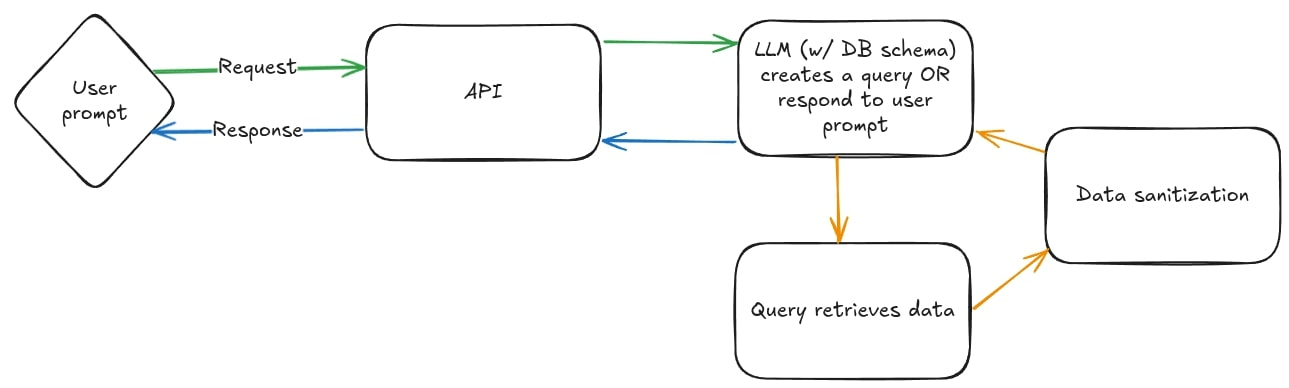
\includegraphics[keepaspectratio]{images/orm/orm-diagram-approach.jpg}}
\caption{ORM - Diagrama da Arquitetura}
\end{figure}

O fluxo de comunicação se inicia com uma solicitação do usuário em
linguagem natural, que é processada pelo LLM. O modelo, tendo
conhecimento prévio do esquema do banco de dados, gera consultas SQL
apropriadas. Estas consultas são executadas no banco de dados, e os
resultados são novamente interpretados pelo LLM para fornecer uma
resposta contextualizada ao usuário.

Em casos mais complexos, o sistema pode realizar múltiplas iterações de
consultas, com o LLM analisando progressivamente os dados até obter
todas as informações necessárias para uma resposta completa.

\paragraph{2.2.2.2 Componentes de
Segurança}\label{componentes-de-seguranuxe7a}

A implementação inclui camadas de segurança essenciais: - Sanitização de
consultas SQL - Controle de acesso em nível de campo - Mascaramento de
dados sensíveis - Validação de permissões de usuário

\paragraph{2.2.2.3 Estrutura de Metadados}\label{estrutura-de-metadados}

A configuração do sistema é gerenciada através de uma estrutura de
metadados que define: - Esquema do banco de dados - Regras de acesso -
Contexto de negócio - Restrições de consulta

\paragraph{2.2.2.4 Implementação da Prova de
Conceito}\label{implementauxe7uxe3o-da-prova-de-conceito}

A implementação utiliza uma stack tecnológica moderna baseada em
Node.js, escolhida por sua eficiência e amplo suporte a ferramentas de
desenvolvimento. Os principais componentes tecnológicos incluem:

\begin{itemize}
\tightlist
\item
  Backend: Node.js
\item
  LLM: GPT-3 via API OpenAI
\item
  Banco de Dados: PostgreSQL
\item
  ORM: Sequelize
\end{itemize}

\paragraph{2.2.2.5 Desenvolvimento do
Conector}\label{desenvolvimento-do-conector}

O conector de banco de dados é implementado utilizando o Sequelize ORM,
que facilita: - Introspection do esquema do banco - Construção dinâmica
de queries - Gerenciamento de conexões - Validação de dados

\paragraph{2.2.2.6 Detalhes Técnicos}\label{detalhes-tuxe9cnicos}

A implementação técnica foca em três aspectos principais:

\paragraph{2.2.2.7 Integração com LLM}\label{integrauxe7uxe3o-com-llm}

O sistema utiliza técnicas avançadas de prompt engineering para: -
Geração precisa de SQL - Manutenção de contexto do esquema - Otimização
de consultas - Interpretação de resultados

\paragraph{2.2.2.8 Tratamento de Erros}\label{tratamento-de-erros}

O sistema implementa estratégias robustas para: - Erros de execução de
queries - Falhas de interpretação do LLM - Timeout de conexões - Dados
inconsistentes

\paragraph{2.2.2.9 Avaliação e
Métricas}\label{avaliauxe7uxe3o-e-muxe9tricas}

A avaliação da solução é realizada considerando:

\paragraph{2.2.2.10 Performance}\label{performance}

\begin{itemize}
\tightlist
\item
  Tempo de resposta médio
\item
  Latência de processamento LLM
\item
  Eficiência de queries
\end{itemize}

\paragraph{2.2.2.11 Segurança}\label{seguranuxe7a}

\begin{itemize}
\tightlist
\item
  Efetividade do controle de acesso
\item
  Prevenção de injeção SQL
\item
  Conformidade com práticas de privacidade
\end{itemize}

\paragraph{2.2.2.12 Custos Operacionais}\label{custos-operacionais}

\begin{itemize}
\tightlist
\item
  Consumo de API do LLM
\item
  Recursos de banco de dados
\item
  Infraestrutura necessária
\end{itemize}

\paragraph{2.2.2.13 Considerações
Práticas}\label{considerauxe7uxf5es-pruxe1ticas}

A implementação revelou diversos aspectos práticos importantes:

\paragraph{2.2.2.14 Desafios}\label{desafios}

\begin{itemize}
\tightlist
\item
  Complexidade de queries dinâmicas
\item
  Limitações do LLM
\item
  Gestão de estados e contexto
\end{itemize}

\paragraph{2.2.2.15 Infraestrutura}\label{infraestrutura}

\begin{itemize}
\tightlist
\item
  Requisitos de escalabilidade
\item
  Arquitetura de deployment
\item
  Monitoramento e logging
\end{itemize}

\paragraph{2.2.2.16 Manutenção}\label{manutenuxe7uxe3o}

\begin{itemize}
\tightlist
\item
  Atualizações de esquema
\item
  Versionamento de modelos
\item
  Monitoramento de performance
\end{itemize}

\section{3 RESULTADOS E DISCUSSÕES}\label{resultados-e-discussuxf5es}

Nos Resultados e Discussões, deve-se apresentar os resultados obtidos no
Procedimento Experimental e fazer uma discussão e análise sobre os
mesmos sempre que possível referenciando a literatura pesquisada.

\section{4 CONSIDERAÇÕES FINAIS}\label{considerauxe7uxf5es-finais}

Etapa esta que servirá para você evidenciar as conquistas alcançadas com
o estudo e indicar as limitações e as reconsiderações. Além disso, você
poderá apontar a relação entre fatos verificados e teoria e mostrar a
contribuição da pesquisa para o meio acadêmico, empresarial e/ou para o
desenvolvimento da ciência e tecnologia. Além disso, você poderá sugerir
temas complementares a sua pesquisa para estudos futuros. Responda aqui
a sua pergunta-problema de pesquisa.

\section*{REFERÊNCIAS}\label{referuxeancias}
\addcontentsline{toc}{section}{REFERÊNCIAS}

\phantomsection\label{refs}
\begin{CSLReferences}{0}{1}
\bibitem[\citeproctext]{ref-anthropic2024context}
ANTHROPIC. \textbf{Anthropic Now Offers 100K Context Windows for Claude
3 Models}. Disponível em:
\textless{}\url{https://www.anthropic.com/news/100k-context-windows}\textgreater.

\bibitem[\citeproctext]{ref-anthropic2024mcp}
ANTHROPIC. \textbf{Model Context Protocol (MCP): A Standard for AI
Context Integration}. Disponível em:
\textless{}\url{https://www.anthropic.com/news/model-context-protocol}\textgreater.
Acesso em: 12 abr. 2025b.

\bibitem[\citeproctext]{ref-Anthropic2024}
ANTHROPIC. \textbf{{Introducing the Model Context Protocol}}. Anthropic
News, nov. c2024. Disponível em:
\textless{}\url{https://www.anthropic.com/news/model-context-protocol}\textgreater{}

\bibitem[\citeproctext]{ref-RedHat2024LLMNode}
BLOG, R. H. D. \textbf{Building LLM Agents with Node.js}.
\url{https://developers.redhat.com/blog/2024/10/25/building-agents-large-language-modelsllms-and-nodejs},
2024.

\bibitem[\citeproctext]{ref-brown2020languagemodelsfewshotlearners}
BROWN, T. B. et al. \textbf{Language Models are Few-Shot Learners}.,
2020. Disponível em:
\textless{}\url{https://arxiv.org/abs/2005.14165}\textgreater{}

\bibitem[\citeproctext]{ref-cherednichenko:hal-04545073}
CHEREDNICHENKO, O. et al. \textbf{Selection of Large Language Model for
development of Interactive Chat Bot for SaaS Solutions}. Lviv, Ukraine:
abr. 2024. Disponível em:
\textless{}\url{https://hal.science/hal-04545073}\textgreater{}

\bibitem[\citeproctext]{ref-Deng2023AMA}
DENG, X. \href{https://api.semanticscholar.org/CorpusID:258259387}{A
More Accessible Web with Natural Language Interface}.
\textbf{Proceedings of the 20th International Web for All Conference},
2023.

\bibitem[\citeproctext]{ref-enterprisedb2023security}
ENTERPRISEDB. \textbf{EnterpriseDB Raises the Bar for Postgres Security
and Compliance}. Disponível em:
\textless{}\url{https://www.enterprisedb.com/news/enterprisedb-raises-bar-postgres-security-compliance}\textgreater.
Acesso em: 12 abr. 2025b.

\bibitem[\citeproctext]{ref-enterprisedb2023postgresql}
ENTERPRISEDB. \textbf{Postgres is the Most Admired Database in Stack
Overflow 2023 Survey}. Disponível em:
\textless{}\url{https://www.enterprisedb.com/blog/postgres-most-admired-database-in-stack-overflow-2023}\textgreater.
Acesso em: 12 abr. 2025a.

\bibitem[\citeproctext]{ref-HuggingFace2024}
FACE, H. \textbf{JavaScript Libraries for ML Integration}.
\url{https://huggingface.co/docs/huggingface.js/}, 2024.

\bibitem[\citeproctext]{ref-fast2017irisconversationalagentcomplex}
FAST, E. et al. \textbf{Iris: A Conversational Agent for Complex
Tasks}., 2017. Disponível em:
\textless{}\url{https://arxiv.org/abs/1707.05015}\textgreater{}

\bibitem[\citeproctext]{ref-Guo2024Doppelganger}
GUO, S. et al. \textbf{Collaborating with my Doppelgänger: The Effects
of Self-similar Appearance and Voice of a Virtual Character during a
Jigsaw Puzzle Co-solving Task}. Proceedings of the ACM on Computer
Graphics and Interactive Techniques. \textbf{Anais}...2024. Disponível
em:
\textless{}\url{https://www.researchgate.net/publication/335223260_The_Effects_of_Continuous_Conversation_and_Task_Complexity_on_Usability_of_an_AI-Based_Conversational_Agent_in_Smart_Home_Environments}\textgreater{}

\bibitem[\citeproctext]{ref-IBM2023WatsonxSDK}
IBM. \textbf{IBM Generative AI Node.js SDK}.
\url{https://github.com/IBM/ibm-generative-ai-node-sdk}, 2023.

\bibitem[\citeproctext]{ref-inie2025summon}
INIE, N.; STRAY, J.; DERCZYNSKI, L.
\href{https://journals.plos.org/plosone/article?id=10.1371/journal.pone.0314658}{Summon
a demon and bind it: A grounded theory of LLM red teaming}. \textbf{PloS
one}, v. 20, n. 1, p. e0314658, 2025.

\bibitem[\citeproctext]{ref-john2025owasp}
JOHN, S. et al.
\textbf{\href{https://genai.owasp.org/llmrisk/llm01-prompt-injection}{OWASP
Top 10 for LLM Apps \& Gen AI Agentic Security Initiative}}. tese de
doutorado---{[}s.l.{]} OWASP, 2025.

\bibitem[\citeproctext]{ref-Kocaballi2019}
KOCABALLI, A. B. et al. \href{https://doi.org/10.2196/15360}{The
Personalization of Conversational Agents in Health Care: Systematic
Review}. \textbf{J Med Internet Res}, v. 21, n. 11, p. e15360, 7 nov.
2019.

\bibitem[\citeproctext]{ref-Lister2020AccessibleCU}
LISTER, K. et al.
\href{https://api.semanticscholar.org/CorpusID:218539971}{Accessible
conversational user interfaces: considerations for design}.
\textbf{Proceedings of the 17th International Web for All Conference},
2020.

\bibitem[\citeproctext]{ref-MCPDocs2024}
MODEL CONTEXT PROTOCOL CONTRIBUTORS. \textbf{{Model Context Protocol
Documentation - Introduction}}. Online Documentation, 2024. Disponível
em:
\textless{}\url{https://modelcontextprotocol.io/introduction}\textgreater{}

\bibitem[\citeproctext]{ref-mcp2025spec}
MODEL CONTEXT PROTOCOL TEAM. \textbf{Model Context Protocol
Specification}. {[}s.l.{]} Model Context Protocol, 26 mar. 2025.
Disponível em:
\textless{}\url{https://modelcontextprotocol.io/specification/2025-03-26/index}\textgreater.
Acesso em: 12 abr. 2025.

\bibitem[\citeproctext]{ref-Nodejs2024Docs}
NODE.JS. \textbf{Streams, Pipelines and WebSocket support}.
\url{https://nodejs.org/api/stream.html}, 2024.

\bibitem[\citeproctext]{ref-openai2022instructgpt}
OPENAI. \textbf{Aligning Language Models to Follow Instructions}.
{[}s.l.{]} OpenAI, 27 jan. 2022. Disponível em:
\textless{}\url{https://openai.com/index/instruction-following/}\textgreater.
Acesso em: 12 abr. 2025.

\bibitem[\citeproctext]{ref-openai2023gpt4}
OPENAI. \textbf{GPT-4 Research}. {[}s.l.{]} OpenAI, a2023. Disponível
em:
\textless{}\url{https://openai.com/index/gpt-4-research/}\textgreater.

\bibitem[\citeproctext]{ref-openai2023functioncalling}
OPENAI. \textbf{Function Calling and Other API Updates}. Disponível em:
\textless{}\url{https://openai.com/index/function-calling-and-other-api-updates/}\textgreater.
Acesso em: 12 abr. 2025b.

\bibitem[\citeproctext]{ref-OpenAI2023}
OPENAI. \textbf{{ChatGPT plugins}}. OpenAI Product Blog, mar. c2023.
Disponível em:
\textless{}\url{https://openai.com/blog/chatgpt-plugins}\textgreater{}

\bibitem[\citeproctext]{ref-OpenAPIInitiative2023}
OPENAPI INITIATIVE. \textbf{{OpenAPI Specification - Getting Started}}.
OpenAPI Documentation (openapis.org), 2023. Disponível em:
\textless{}\url{https://learn.openapis.org/docs/getting-started}\textgreater{}

\bibitem[\citeproctext]{ref-oprea2023adversarial}
OPREA, A.; VASSILEV, A. \textbf{Adversarial machine learning: A taxonomy
and terminology of attacks and mitigations}. {[}s.l.{]} National
Institute of Standards; Technology, 2023. Disponível em:
\textless{}\url{https://csrc.nist.gov/pubs/ai/100/2/e2023/final}\textgreater.

\bibitem[\citeproctext]{ref-RAPP201849}
RAPP, A. et al.
\href{https://doi.org/10.1016/j.ijhcs.2018.07.005}{Designing technology
for spatial needs: Routines, control and social competences of people
with autism}. \textbf{International Journal of Human-Computer Studies},
v. 120, p. 49--65, 2018.

\bibitem[\citeproctext]{ref-ribeiro2020beyond}
RIBEIRO, M. T. et al. \href{https://arxiv.org/abs/2005.04118}{Beyond
accuracy: Behavioral testing of NLP models with CheckList}.
\textbf{arXiv preprint arXiv:2005.04118}, 2020.

\bibitem[\citeproctext]{ref-eversql2023orms}
TEAM, E. \textbf{Best ORM for Node.js in 2023: A Comprehensive
Comparison}. Disponível em:
\textless{}\url{https://www.eversql.com/best-orm-for-node-js/}\textgreater.
Acesso em: 12 abr. 2025.

\bibitem[\citeproctext]{ref-sequelize2024}
TEAM, S. \textbf{Sequelize: A Modern TypeScript and Node.js ORM for
Postgres, MySQL, MariaDB, SQLite and SQL Server}., 2024. Disponível em:
\textless{}\url{https://github.com/sequelize/sequelize}\textgreater.
Acesso em: 12 abr. 2025

\bibitem[\citeproctext]{ref-Postman2023}
THE POSTMAN TEAM. \textbf{{What is OpenAPI?}} Postman Blog, ago. 2023.
Disponível em:
\textless{}\url{https://blog.postman.com/what-is-openapi/}\textgreater{}

\bibitem[\citeproctext]{ref-wei2023chainofthoughtpromptingelicitsreasoning}
WEI, J. et al. \textbf{Chain-of-Thought Prompting Elicits Reasoning in
Large Language Models}., 2023. Disponível em:
\textless{}\url{https://arxiv.org/abs/2201.11903}\textgreater{}

\bibitem[\citeproctext]{ref-wu2023defending}
WU, F. et al.
\href{https://www.researchsquare.com/article/rs-2873090/v1}{Defending
chatgpt against jailbreak attack via self-reminder}. 2023.

\bibitem[\citeproctext]{ref-yao2023treethoughtsdeliberateproblem}
YAO, S. et al. \textbf{Tree of Thoughts: Deliberate Problem Solving with
Large Language Models}., 2023. Disponível em:
\textless{}\url{https://arxiv.org/abs/2305.10601}\textgreater{}

\bibitem[\citeproctext]{ref-Zhu2025DyT}
ZHU, J. et al. \textbf{Transformers without Normalization}. Proceedings
of the IEEE/CVF Conference on Computer Vision and Pattern Recognition
(CVPR). \textbf{Anais}...2025.

\end{CSLReferences}

\end{document}
